\documentclass[12pt]{article}
\usepackage{amsmath}
\usepackage{amsfonts}
\usepackage{parskip}
\usepackage{amsthm}
\usepackage{thmtools}
\usepackage[headheight=15pt]{geometry}
\geometry{a4paper, left=20mm, right=20mm, top=30mm, bottom=30mm}
\usepackage{graphicx}
\usepackage{bm} % for bold font in math mode - command is \bm{text}
\usepackage{enumitem}
\usepackage{fancyhdr}
\usepackage{amssymb} % for stacked arrows and other shit
\pagestyle{fancy}
\usepackage{changepage}
\usepackage{mathcomp}
\usepackage{tcolorbox}
\usepackage{caption}
\usepackage{subcaption}

\linespread{1.3}

\declaretheoremstyle[headfont=\normalfont]{normal}
\declaretheorem[style=normal]{Theorem}
\declaretheorem[style=normal]{Proposition}
\declaretheorem[style=normal]{Lemma}
\newcounter{ProofCounter}
\newcounter{ClaimCounter}[ProofCounter]
\newcounter{SubClaimCounter}[ClaimCounter]
\newenvironment{Proof}{\stepcounter{ProofCounter}\textsc{Proof.}}{\hfill$\square$}
\newenvironment{claim}[1]{\vspace{1mm}\stepcounter{ClaimCounter}\par\noindent\underline{\bf Claim \theClaimCounter:}\space#1}{}
\newenvironment{claimproof}[1]{\par\noindent\underline{Proof of claim \theClaimCounter:}\space#1}{\hfill $\blacksquare$ Claim \theClaimCounter}
\newenvironment{subclaim}[1]{\stepcounter{SubClaimCounter}\par\noindent\emph{Subclaim \theClaimCounter.\theSubClaimCounter:}\space#1}{}
% \newenvironment{subclaimproof}[1]{\begin{adjustwidth}{2em}{0pt}\par\noindent\emph{Proof of subclaim \theClaimCounter.\theSubClaimCounter:}\space#1}{\hfill
% $\blacksquare$ \emph{Subclaim \theClaimCounter.\theSubClaimCounter}\vspace{5mm}\end{adjustwidth}}
\newenvironment{subclaimproof}[1]{\par\noindent\emph{Proof of subclaim \theClaimCounter.\theSubClaimCounter:}\space#1}{\hfill
$\Diamond$ \emph{Subclaim \theClaimCounter.\theSubClaimCounter}}

\allowdisplaybreaks{}

% chktex-file 3

\title{STAT 520: Assignment 4}
\author{Evan P. Walsh}
\makeatletter
\makeatother
\lhead{Evan P. Walsh}
\chead{STAT 520: Assignment 4}
\rhead{\thepage}
\cfoot{}

\begin{document}
% \maketitle

\subsection*{Nitrate Concentrations in Drinking Water}

Drinking water was sampled from individual wells in three different counties in Iowa, with 25 wells sampled from each county. In each well the nitrate
concentration was measured since nitrate is considered to be a contaminate, with concentrations above 5 being an indication of risk.
We are interested in whether there are differences in the distributions of nitrate concentration across wells for the three different counties.
Figure \ref{boxplot} shows side-by-side boxplots of the nitrate concentrations in the wells for each county, and Figure \ref{density} shows the empirical density
functions of the nitrate concentrations in the wells for each county.

\begin{figure}[h]
  \caption{\emph{Side-by-side boxplots of the nitrate concentrations in each county.}}
  \centering
  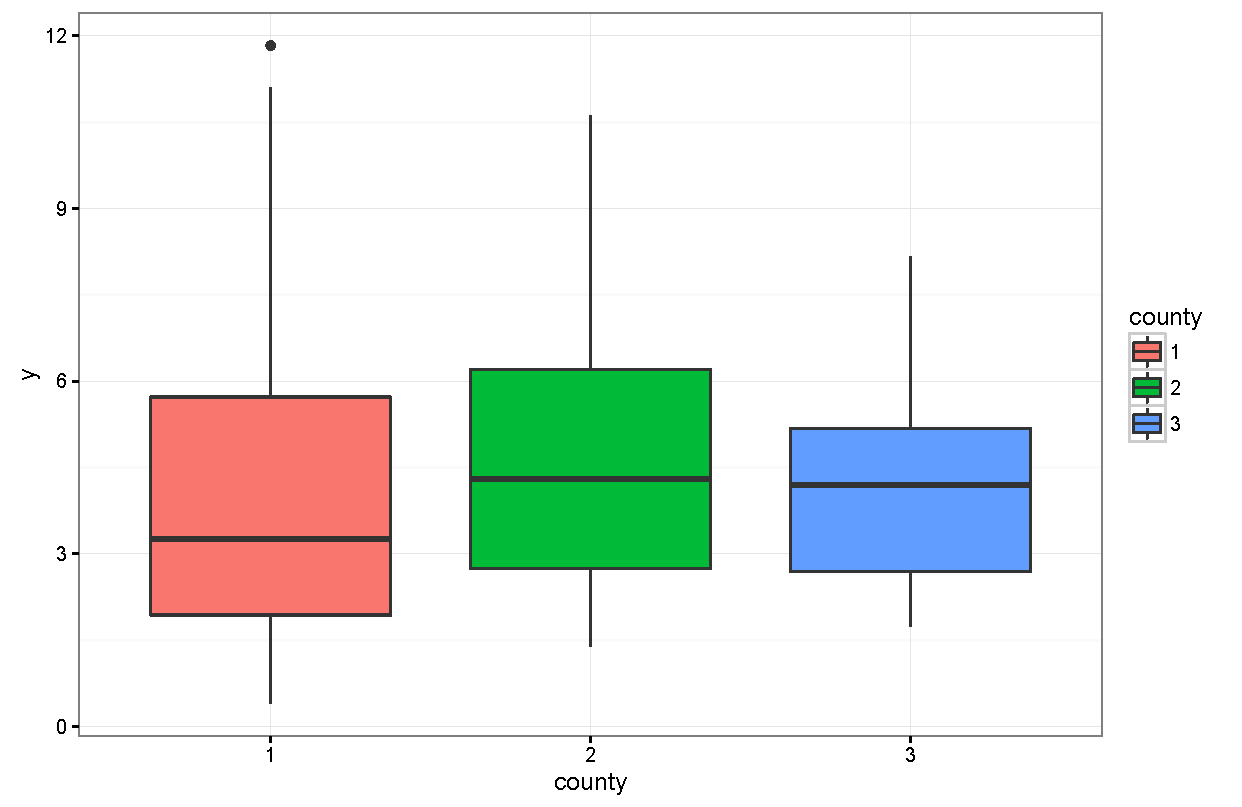
\includegraphics[width=.7\textwidth]{./figures/hw04_boxplots.pdf}
  \label{boxplot}
\end{figure}

\begin{figure}[h]
  \caption{\emph{Empirical density curves of the nitrate concentrations in each county.}}
  \centering
  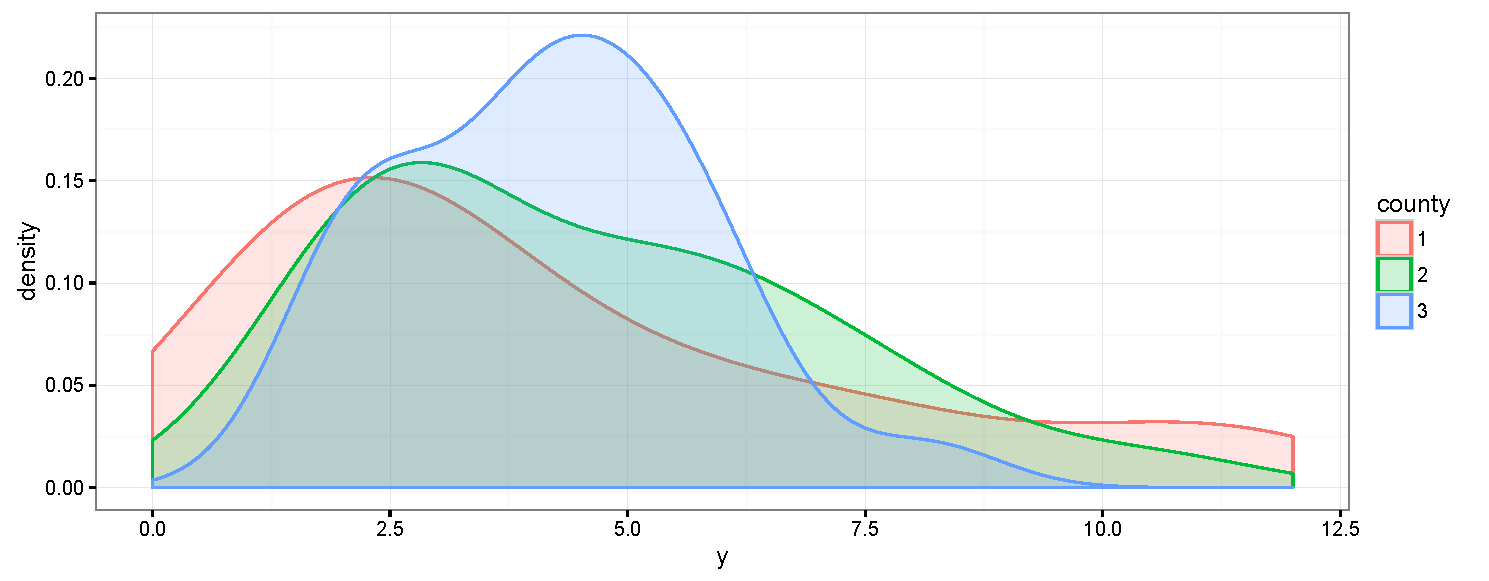
\includegraphics[width=.9\textwidth]{./figures/hw04_density.pdf}
  \label{density}
\end{figure}

\newpage

\begin{enumerate}
  \item We define the random variables $Y_{1}, \dots, Y_{75}$ where $Y_{i}$ is associated with the nitrate concentration in mg/L of the $i^{th}$ well.
    We also define the covariates $x_{i,j}$, for $i = 1,
    \hdots, 75$ and $j = 1,2$, where
    \[
      x_{i,j} := \left\{ \begin{array}{cl}
          1 & \text{ if the $i^{th}$ well is in county $j$,} \\
          0 & \text{ otherwise}.
      \end{array} \right.
    \]
    Note that we only need two covariates here and not three since we will fit the model with an intercept.
    Since the covariates are just dummy variables for group membership, the particular form of the link function will no effect on the model in terms
    of inference for the expected value and variance of each distribution.
    Thus we simply choose to use the canonical link function for the Gamma distribution: $g(\mu_i) := 1 / \mu_i$.
    

    \begin{table}[h]
      \caption{\emph{Results of a glm fit to the nitrate concentrations in each well with a Gamma random component and the Gamma canonical link.
      $\hat{\phi}$ is the usual method of moments estimator of the dispersion parameter $\phi$.}}
      \vspace{.2cm}
      \centering
      \begin{tabular}{|c|c|c|c|}
        \hline
        $\hat{\phi}$ & Unscaled deviance & Scaled deviance & $\ell(\hat{\beta_0}, \hat{\beta_1}, \hat{\beta_2}, \hat{\phi})$ \\
        \hline
        2.9542 & 26.1672 & 77.3024 & $-69.0587$ \\
        \hline
      \end{tabular}
      \label{tab:1}
    \end{table}


    \begin{table}[h]
      \caption{\emph{Parameter estimates, standard errors, and 95\% Wald theory confidence intervals. Here the $\beta$'s are the coefficients for the
      systematic (linear) component in our model, not the rate parameter in a Gamma distribution.}}
      \vspace{.2cm}
      \centering
      \begin{tabular}{|c|c|c|c|}
        \hline
        Parameter & Estimate & Standard error & 95\% CI \\
        \hline
        $\beta_0$ & 0.2386 & 0.0278 & $(0.1842,0.2930)$ \\
        \hline
        $\beta_1$ & $-0.0029$ & 0.0390 & $(-0.0794, 0.0736)$ \\
        \hline
        $\beta_2$ & $-0.0201$ & 0.0376 & $(-0.0939, 0.0537)$ \\
        \hline
      \end{tabular}
      \label{tab:2}
    \end{table}

    Table 1 and Table 2 report the results of fitting the generalized linear model just described using the R function \texttt{glm}.
    We use the fact that maximum likelihood estimates are asymptically normal with a covariance matrix that can be approximated by the inverse of
    the observed Fisher information matrix to construct 95\% confidence intervals for the true coefficients $\beta_{j}$, $j = 0, 1, 2$.

    Note that the implicit assumption of our model was that the ``shape'' parameter for each distribution was equal to $\phi$, the dispersion
    parameter. That is, $\alpha_i \equiv \phi$ for all $i = 1, \dots, 75$. Thus the distributions are only allowed to differ through the ``rate''
    parameter $\beta$. With blatant abuse of notation we now define $\beta_j$, for $j = 1, 2, 3$, to be the ``rate'' parameter for the distribution of
    the nitrate concentrations across wells in county $j$. 
    
    Using the multivariate delta method with Slutsky's Theorem and the fact that the method of
    moments estimator of $\phi$ is consistent, we can construct confidence intervals for pairwise differences in the $\beta_{j}$'s.
    The results of this analysis are shown in Table 3.

    \begin{table}[h]
      \caption{\emph{Estimates of the rate parameters for the distributions of the nitrate concentration across wells in each county.}}
      \vspace{.5cm}
      \centering
      \begin{tabular}{|c|c|c|}
        \hline
        Parameter & Estimate & 95\% CI \\
        \hline
        $\beta_1$ & 0.6963 & $(0.5375,0.8551)$ \\
        \hline
        $\beta_2$ & 0.6369 & $(0.3672, 0.9065)$ \\
        \hline
        $\beta_3$ & 0.7048 & $(0.5440, 0.8655)$ \\
        \hline
        $\beta_1 - \beta_2$ & 0.0509 & $(-0.1656, 0.2674)$ \\
        \hline
        $\beta_1 - \beta_3$ & $-0.0085$ & $(-0.2345, 0.2174)$ \\
        \hline
        $\beta_2 - \beta_3$ & $-0.0594$ & $(-0.2774, 0.1585)$ \\
        \hline
      \end{tabular}
      \label{tab:3}
    \end{table}

    Since all of the confidence intervals for the pairwise differences in the estimated ``rate'' parameters contain 0, there is not sufficient
    evidence to believe the distributions for the nitrate concentration across wells in the three counties are different. An estimate of the common
    distribution function is shown in Figure \ref{combined_density}. Using this estimated common distribution with $\hat{\alpha} = \hat{\phi} = 3.0311$ and
    $\hat{\beta} = 0.6793$, we calculate that the probability of a randomly chosen well from any of the three counties having a nitrate concentration of less
    than 3 mg/L is 0.342 and more than 10 mg/L is 0.031.


    \begin{figure}[h]
      \caption{\emph{Estimated common density function for the distribution of nitrate concentration.}}
      \centering
      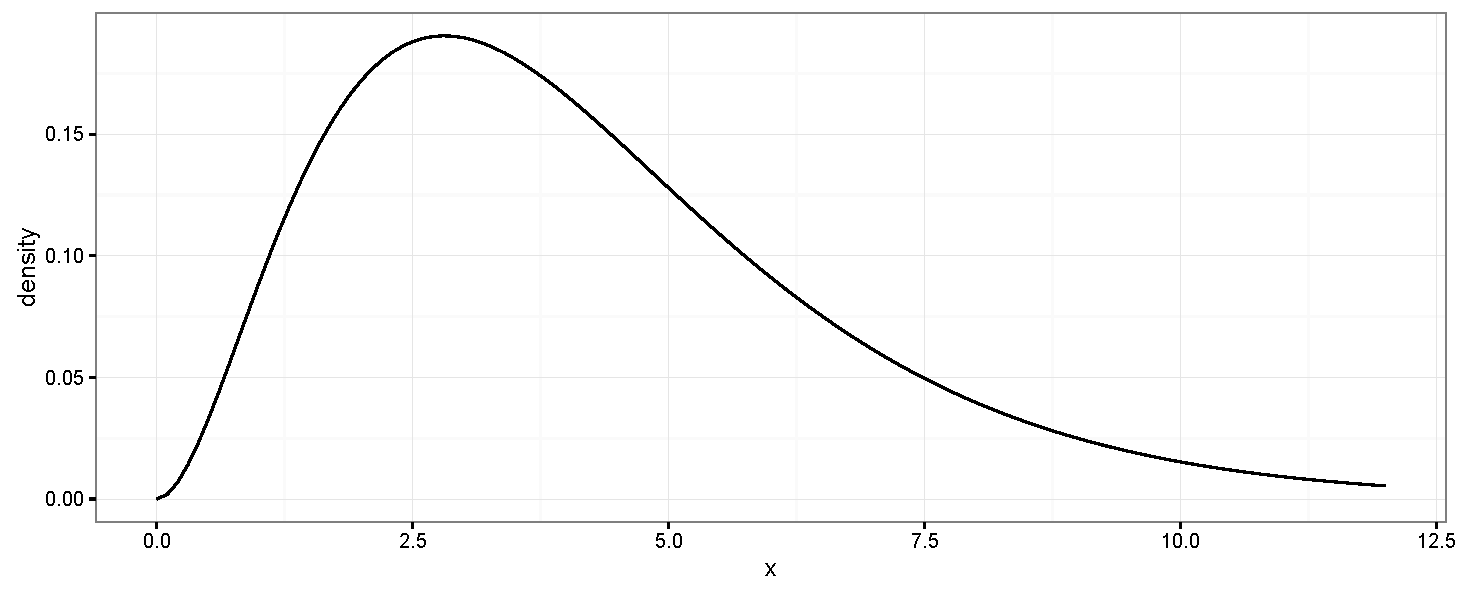
\includegraphics[width=.95\textwidth]{./figures/hw04_combined_density.pdf}
      \label{combined_density}
    \end{figure}

    \newpage

  \item We now attempt to analyze this problem in the context of a likelihood comparison of the three groups. We define the random variables
    $\{Y_{i,j}\}_{i,j}$, for $i = 1, 2, 3$ and $j = 1, \hdots, 25$, such that $Y_{i,j}$ is associated with the nitrate concentrations in mg/L of the water in
    the $j^{th}$ well of the $i^{th}$ county. For all we know, it is perfectly reasonable to treat all the random variables as independent. 

    Naturally we define the full model to consist of three distinct Gamma distributions, one for each county, and the reduced model to consist of a 
    single Gamma distribution for all of the wells. We define $\alpha_i$ and $\beta_i$
    to be the ``shape'' and ``rate'' parameters of the distribution for county $i$, respectively. Hence, for county $i$, the log likelihood function 
    in the full model is given by
    \begin{align*}
      \ell(\alpha_i,\beta_i|y_{i,1},\hdots, y_{i,25}) & = \log\left\{ \prod_{j=1}^{25} \frac{\beta_{i}^{\alpha_i}}{\Gamma(\alpha_i)}y_{i,j}^{\alpha_i - 1} \exp(-\beta_i
      y_{i,j}) \right\} \\
      & = 25 \alpha_i \log(\beta_i) - 25 \log[\Gamma(\alpha_i)] - \beta_i \sum_{j=1}^{25}y_{i,j} + (\alpha_i - 1)\sum_{j=1}^{25}\log(y_{i,j}).
    \end{align*}

    We use the Newton-Raphson method to find maximum likelihood estimates of $\alpha_i$ and $\beta_i$ for each county and for the reduced model with the R fuction
    \texttt{newtraph}. The estimated parameters along with 95\% Wald theory confidence intervals are displayed in Table 4.

    \begin{table}[h]
      \caption{\emph{MLE estimates and 95\% Wald theory confidence intervals.}}
      \centering
      \begin{tabular}{|l|c|c|c|c|}
        \hline
        & $\hat{\alpha}$ & 95\% Wald CI for $\alpha$ & $\hat{\beta}$ & 95\% Wald CI for $\beta$ \\
        \hline 
        County 1 & 1.7781 & (0.8697, 2.6865) & 0.4191 & (0.1720, 0.6661) \\
        \hline
        County 2 & 3.7582 & (1.7604, 5.7561) & 0.8210 & (0.3541, 1.2880) \\
        \hline
        County 3 & 6.6032 & (3.0313, 10.1752) & 1.5754 & (0.6900, 2.4608) \\
        \hline
        Reduced & 3.0100 & (2.0950, 3.9251) & 0.6940 & (0.4644, 0.9236) \\
        \hline
      \end{tabular}
    \end{table}

    To test whether the distributions for the counties are significantly different, we compute the test statistic
    \[
      T := -2\left\{ \ell_{R} - \ell_{F} \right\} = -2\left\{ -166.1239 - (-160.0177) \right\} = 12.2125.
    \]
    where $\ell_{R}$ is the log likelihood evaluated at the estimates of the parameters for the reduced model with a single group and $\ell_{F}$ is
    the log likelihood evaluated at the estimates for the full model with three distinct groups. Under the null hypothesis that the there is only one
    distribution for all three counties, $T$ has a limiting distribution of a $\chi_{4}^{2}$ random variable. The 4 degrees of freedom come from the
    difference in dimensionality of the full parameter space ($d = 6$) and the reduced parameter space ($d = 2$). The p-value obtained by computing
    the probability that a $\chi_{4}^{2}$ random variable is greater than $T$ is 0.0158. Thus there is significant evidence to believe the that the
    distributions between the three counties are not all the same.

    The estimated probabilities that the nitrate concentration of a randomly selected well in each county is below 3 mg/L and above 10 mg/L is are
    summarized in Table 5.

    \begin{table}[h]
      \caption{\emph{Estimated probabilities for each county.}}
      \centering
      \begin{tabular}{|c|c|c|}
        \hline
        County & Probability less than 3 mg/L & Probability greater than 10 mg/L \\
        \hline 
        1 & 0.4292 & 0.0587 \\
        \hline
        2 & 0.2786 & 0.0286 \\
        \hline
        3 & 0.2480 & 0.0032 \\
        \hline
      \end{tabular}
    \end{table}

    We also plot the estimated density functions of the nitrate concentration across wells for each county, as shown in Figure \ref{density2}.

    \begin{figure}[h]
      \caption{\emph{Estimated density functions for each county.}}
      \centering
      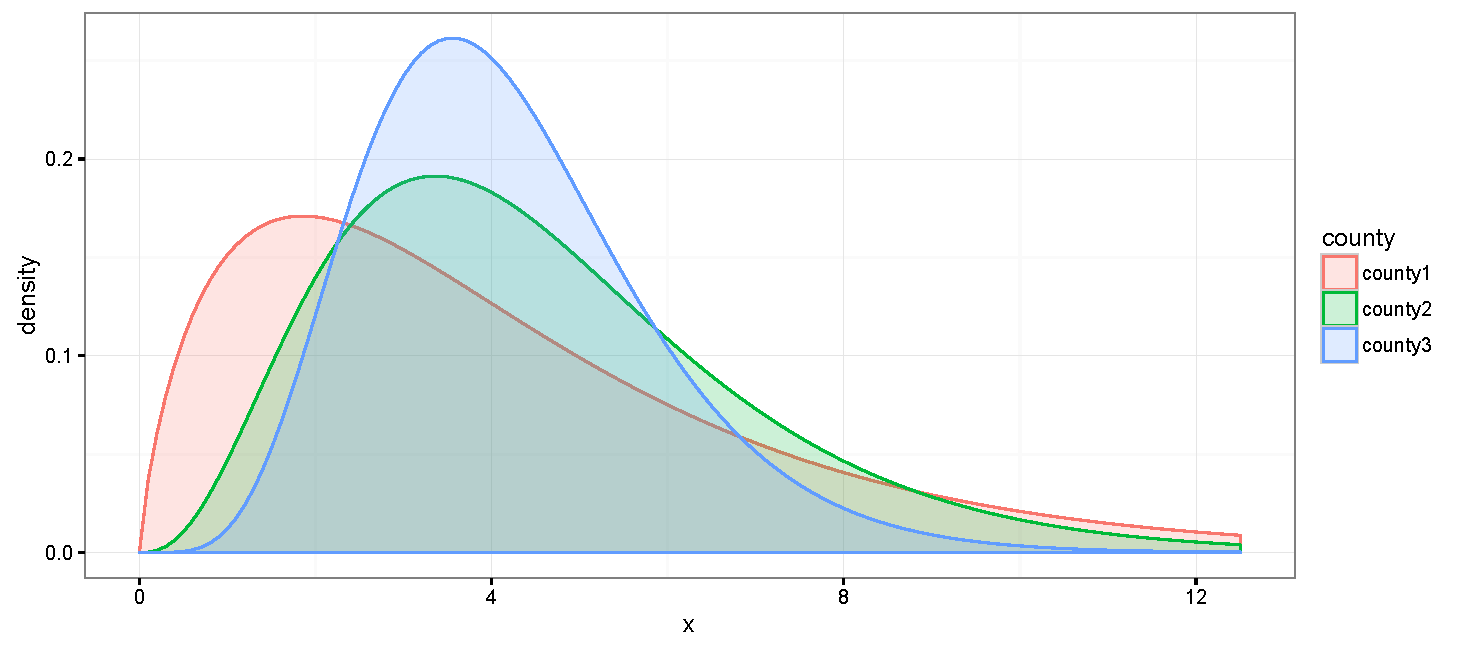
\includegraphics[width=.9\textwidth]{./figures/hw04_density2.pdf}
      \label{density2}
    \end{figure}


  \item The two different approaches to our analysis yielded two different results. When we approached the problem using a generalized linear model,
    we found that there was not significant evidence to believe the distributions of the nitrate concentration across wells was different for
    different counties. However, this analysis relied on the assumption that the shape parameter in each model was the same. 
    On the other hand, when we approached the problem with a likelihood analysis, we found that there was significant evidence in favor a full model which assigned
    different distributions to each county. This suggests that the distributions might vary primarly through the shape parameter $\alpha$.

\end{enumerate}


\end{document}
